%%
%% crosscountry.tex -- Flight Gear documentation: The FlightGear Manual
%% Chapter file
%%
%% Written by Michael Basler, started September 1998.
%%
%% Copyright (C) 2002 Michael Basler
%%
%%
%% This program is free software; you can redistribute it and/or
%% modify it under the terms of the GNU General Public License as
%% published by the Free Software Foundation; either version 2 of the
%% License, or (at your option) any later version.
%%
%% This program is distributed in the hope that it will be useful, but
%% WITHOUT ANY WARRANTY; without even the implied warranty of
%% MERCHANTABILITY or FITNESS FOR A PARTICULAR PURPOSE.  See the GNU
%% General Public License for more details.
%%
%% You should have received a copy of the GNU General Public License
%% along with this program; if not, write to the Free Software
%% Foundation, Inc., 675 Mass Ave, Cambridge, MA 02139, USA.
%%
%% $Id: crosscountry.tex,v 0.1 2005/09/09 michael
%% (Log is kept at end of this file)

%%%%%%%%%%%%%%%%%%%%%%%%%%%%%%%%%%%%%%%%%%%%%%%%%%%%%%%%%%%%%%%%%%%%
\ifchinese
\chapter{{\\}短途转场飞行教程}
\fi
\iffalse
\chapter{A Cross Country Flight Tutorial}
\fi
\label{crosscountry}
%%%%%%%%%%%%%%%%%%%%%%%%%%%%%%%%%%%%%%%%%%%%%%%%%%%%%%%%%%%%%%%%%%%%

%%%%%%%%%%%%%%%%%%%%%%%%%% CHINESE VERSION %%%%%%%%%%%%%%%%%%%%%%%%%

\ifchinese
\section{简介}

\begin{figure}[!htp]
\centering
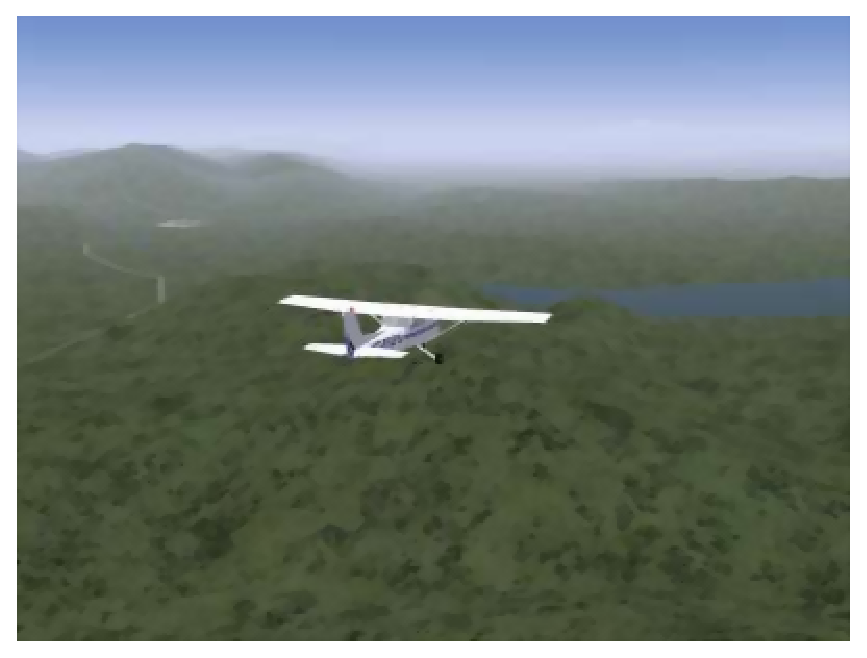
\includegraphics[width=0.5\textwidth]{antonio2}
\caption{从圣安东尼奥大坝飞到利弗莫尔}
\end{figure}

本教程将会模拟一次转场飞行,从里德—晓岚机场(Reid-Hillview,KRHV)到利弗莫尔机场(Livermore,KLVK),使用目视飞行规则(Visual Flight Rules,VFR)。这两个机场都已经包括在了 FlightGear 的基础包里,因此不需要另外安装地景。

我假设你已经学会了 FlightGear 里的起飞、爬升、转弯、下降和降落。否则,建议你看一下之前的教程。本教程基于之前的教程基础,并增加了飞行系统和程序方面更复杂的信息。

\subsection{免责和感谢}

简短的说一句免责。在真实中我是飞 Microlights 的而不是塞斯纳 172。此文中的很多信息从大量非认证的源获取。如果你发现任何错误和误解,请联系我 stuart\_d\_buchanan -at- yahoo.co.uk。

我很想感谢如下这些朋友的帮助,使此教程更精确更深入浅出:Benno Schulenberg, Sid Boyce, Vassilii Khachaturov, James Briggs。

\section{飞行计划}

飞行之前,我们需要先计划一下。否则我们起飞以后都不知道要向哪边转。

首先来看看这一地区的\Index{区域图}。这是一张标示有机场、导航辅助设施及障碍物的地图。VFR 所用的区域图有两种比例尺,分别是 1:500,000 区域图和覆盖某些繁忙空域的 1:250,000 VFR 终端区域图。

都可以在飞行员商店买到,在线的也有很多,比如:

\medskip
\web{http://www.runwayfinder.com/}\footnote{此网站已关闭。可以使用 VFRmap.com 这个网站来查询 VFR / IFR 区域图和终端图,但只支持美国地区。——译者注}
\medskip

只需要搜索 Reid-Hillview 就可以看到如图 ~\ref{sectional} 这样的区域图了。

\begin{figure}[!htp]
\centering
\includegraphics[width=\textwidth]{sectional}
\caption{一张包含里德—晓岚机场和利弗莫尔机场的区域图\label{sectional}}
\end{figure}

如果你需要包含整个地区并显示飞机具体地点的地图,你可以使用 Atlas。这是一个可移动的地图,连接到 FlightGear 上。详情可参考 \ref{Atlas} 小节。

那么我们如何从里德—晓岚机场到利弗莫尔机场呢?

我们要从 KRHV 的 31R 跑道起飞。KRHV 是 \Index{Reid-Hillview 里德—晓岚}机场的 ICAO 四字代码,并可在 FlightGear 的向导里找到。

“31” 表示跑道的磁航向是 310 度,字母“R”表示使用右侧的跑道,从区域图上也可以看到,KRHV 有两条平行的跑道。多条跑道主要是用在交通繁忙的机场,这样每条跑道双向都可以起降。31 跑道从另一个方向看就是 13 跑道。因此可用的跑道就是 13R、13L、31R 和 31L。起飞降落都可以很容易处在顶风方向,因此当风从西北方吹来时,就可以使用跑道 31L 和 31R。跑道入口处会喷涂巨大的跑道号以供飞机在天上识别。

起飞以后,我们会转航向到 350 度直飞\Index{Livermore 利弗莫尔}机场(KLVK)。巡航高度在 3500 英尺,这可以让我们有 500 英尺余量来飞越途中的各种地形和障碍物,比如无线电天线。

我们也会飞过卡拉韦拉斯水库(Calaveras Reservoir)然后是圣安东尼奥水库(San Antonio Reservoir),两个都是巨大的水库,我们可以利用这两个大水库当作地标导航,确保在正确的路径上。

当我们距离利弗莫尔还有 10 英里的时候(飞越圣安东尼奥水库),我们会联系利弗莫尔的空中管制(ATC),获悉我们需要降落在哪里,然后加入机场起落航线并降落。

\section{让我们开始吧}

好了,现在我们已经准备停当了,该开始飞行了。

使用向导启动 FlightGear(用命令行亦可)。我们用 C172P 从圣克拉拉县的里德—晓岚机场(KRHV) 31R 跑道起飞。在佛罗里达飞行,选择黎明会很美。

如果你愿意,可以选择当前真实天气,只需要在向导里勾选“获取真实天气”选项即可。

\begin{figure}[!htp]
\centering
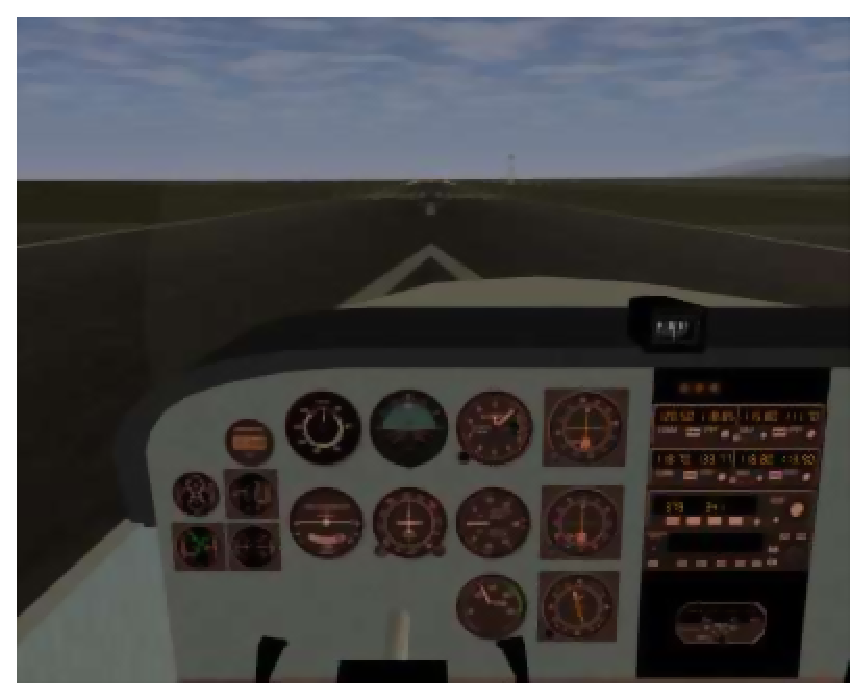
\includegraphics[width=0.5\textwidth]{krhvrunway}
\caption{在 KRHV 的跑道上}
\end{figure}

\subsection{飞行前的程序}

起飞前,我们需要对飞机做起飞前的检查。在真实中,我们需要在飞机周围转一圈,以检查一切部件,并确保油量充足。

在这里,我们要检查天气、设置高度表拨正值并预设一些事情,飞行前来做会比较容易。

天气对飞行来说显然很重要。我们需要知道是否有侧风会影响起飞,以及云的高度(因为是 VFR 飞行,我们需要全程避开云层),任何风都会把我们推出航线。

我们还需要设置高度表拨正值。高度表通过测量当前气压来得知高度,然而天气会影响到气压值,所以高度表读数也会有误差,这在飞越山丘地带时会是致命的。

\subsection{ATIS}

方便的是,机场会通过 \Index{ATIS}\footnote{中国大陆一般将 ATIS 翻译为“机场通播”,本手册中出现 ATIS 的部分,会根据语境,选择不同的翻译文本。——译者注} 广播当前的修正海平面气压,以及有用的天气资讯和机场信息。ATIS 是一条预先录制好的无线电语音信息。为了收听 ATIS,我们需要首先调节无线电。

ATIS 的频率可以在区域图里找到(机场标识旁边的“ATIS”字样),同时也可以在 FlightGear 里找到。要查询机场的频率(包括塔台、地面和进近),使用 ATC/AI 菜单并选择“频率”。然后输入 ICAO 代码(此例是 KRHV),然后机场相关的各种频率信息就会显示出来。如果有多个频率,使用其中之一即可。

好了,里德机场的 ATIS 频率是 125.2MHz。

\subsection{无线电}

现在我们该开始处理\Index{无线电}了。所有无线电相关的都在主仪表板右侧的无线电栈里。实际上有两套独立的无线电系统,1 和 2。每一个无线电又被分成两部分,左侧的是负责无线电通讯的(COMM),右侧则是负责无线电导航的(NAV)。我们这里把 COMM1 的频率设为机场 ATIS 的频率。

\begin{figure}[!htp]
\centering
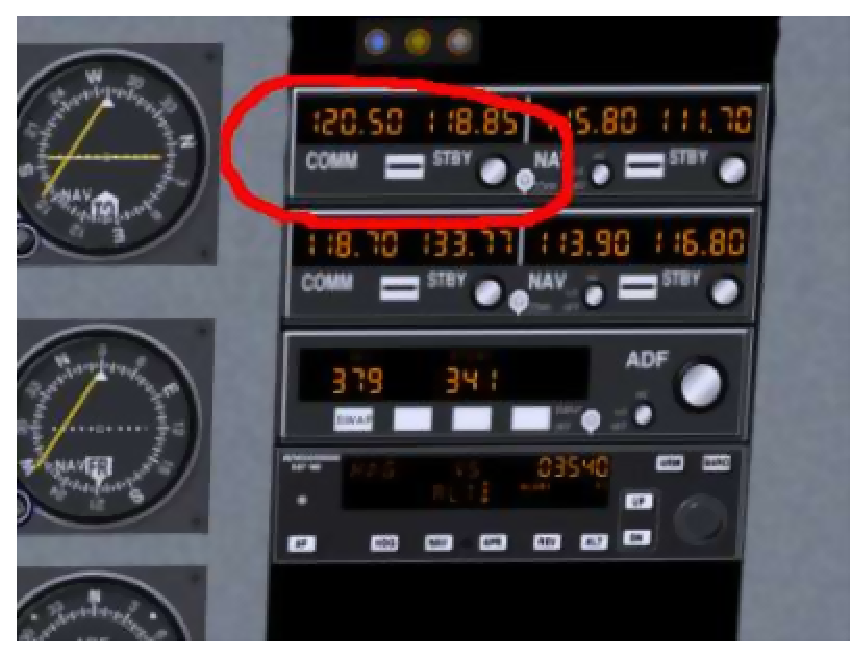
\includegraphics[width=0.5\textwidth]{comm1}
\caption{C172 无线电通讯系统 COMM1 已高亮表示出来\label{comm1}}
\end{figure}

无线电有两套频率。一个是活动频率,也就是正在使用的,另一个是备用频率,表示之后我们将会使用的。左侧的五个数字表示活动频率,而备用频率则在右侧。我们调节备用频率,然后将两者交换,这样备用频率就变成活动频率,相应的活动频率也就变成备用了。这么做可以防止在调节无线电频率时失去联系。

\begin{figure}[!htp]
\centering
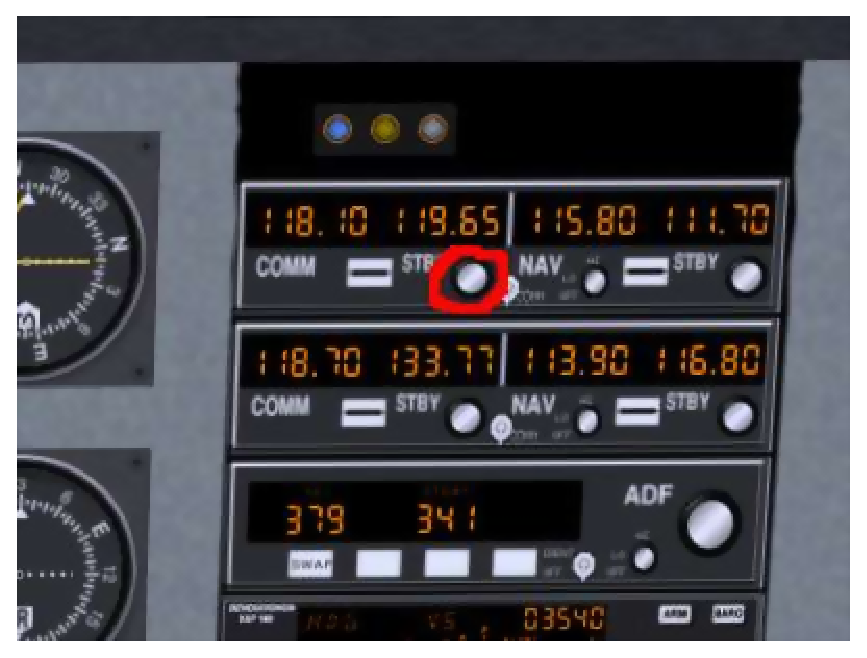
\includegraphics[width=0.5\textwidth]{comm1_knob}
\caption{COMM1 调节旋钮\label{comm1knob}}
\end{figure}

要改变频率,点击备用频率下面的灰色旋钮(也就是图 ~\ref{comm1knob} 标出的部分),就在“STBY”旁边。左键点击可改变小数点后面的数字,鼠标中键点击可改变小数点前边的数字。点击左侧是增加,右侧是减少。FlightGear 里的大多数驾驶舱都是这样操作的。如果你操作有困难,也可以按 CTRL-C 来高亮可操作的区域。

\begin{figure}[!htp]
\centering
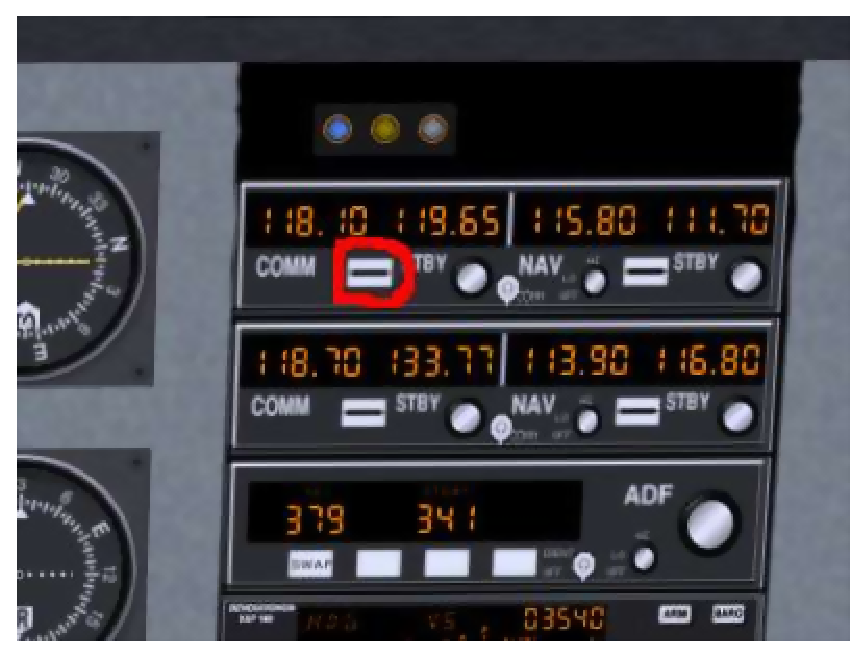
\includegraphics[width=0.5\textwidth]{comm1_switch}
\caption{COMM1 切换开关\label{comm1switch}}
\end{figure}

当频率调到 125.2 之后,按“COMM”和“STBY”之间的那个按钮,来对调活动频率和备用频率(已在图~\ref{comm1switch} 中标出)。很快之后你就可以听到 ATIS 的通播。

\subsection{高度表拨正值和罗盘}

\begin{figure}[!htp]
\centering
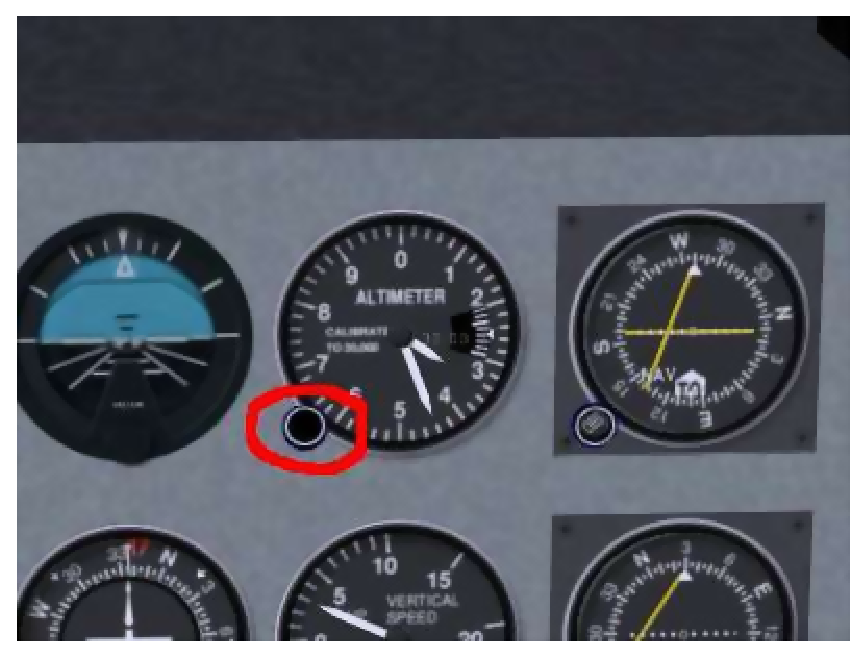
\includegraphics[width=0.5\textwidth]{altimeter}
\caption{高度表拨正值调节旋钮\label{altimeter}}
\end{figure}

仔细收听机场通播(ATIS)里有关“\Index{高度表拨正值(Altimeter)}“相关的内容。如果你没有使用”真实天气“,此值一般是 2992,也就是标准大气压并且已经默认在飞机里设置好。如果你正在使用”真实天气“,高度表拨正值并不一样。因此我们需要将高度表拨正值设定到正确的数值,可以用图~\ref{altimeter} 里圈出的旋钮来调节,方法与之前调节无线电频率相近。高度表上的小窗会显示当前的高度表拨正值,随着拨正值的变化(相当于基准气压改变)高度表的数值也会改变。

另一个方式是检查机场标高,也就是机场与海平面之间的高度。机场标高可在区域图里查到。KRHV 的机场标高是 133 英尺,因此我们可以通过这个数值来交叉检查我们的高度表拨正值。

\begin{figure}[!htp]
\centering
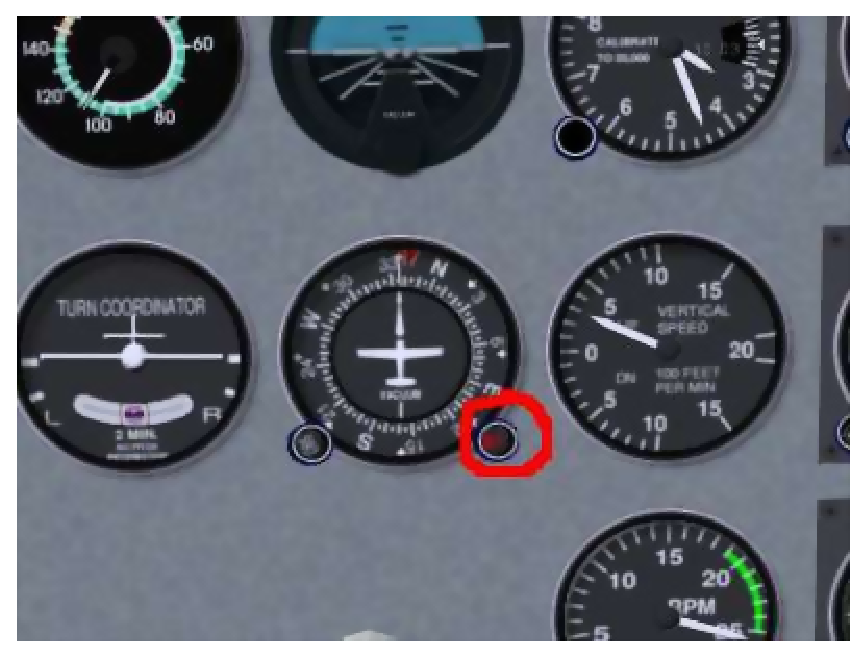
\includegraphics[width=0.5\textwidth]{compass}
\caption{航向调节旋钮\label{head}}
\end{figure}

趁此机会,我们也顺便把罗盘上的航向游标设置在 350——也就是从 KRHV 到 KLVK 的航向。如图~\ref{head},调节罗盘下方的红色旋钮。方式和之前一样,用鼠标左键做小幅调整,用中键做大的改动。350 度只需要逆时针旋转到 N 之后第一个标线的位置即可(N 代表 0 度)

\begin{figure}[!htp]
\centering
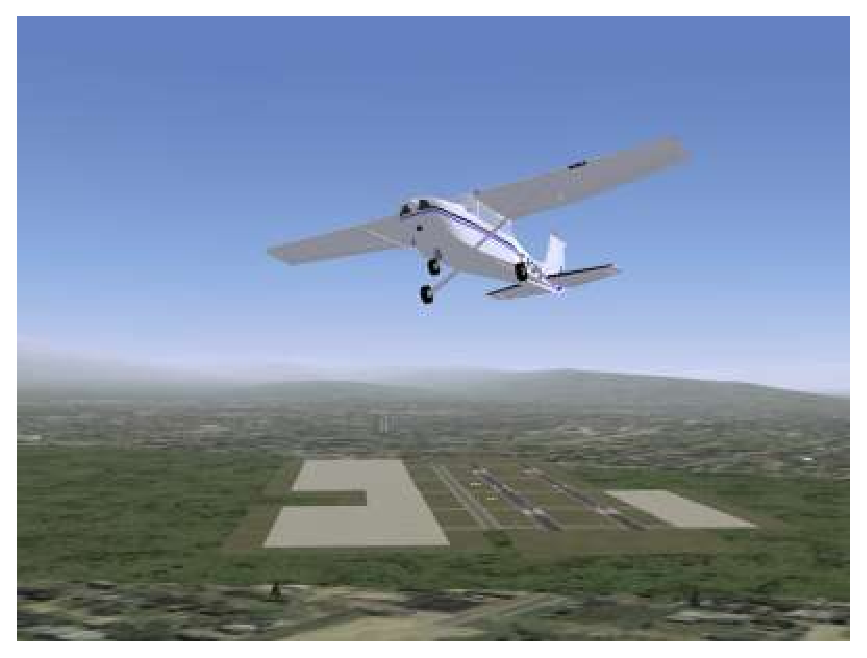
\includegraphics[width=0.5\textwidth]{takeoff}
\caption{从 KRHV 起飞}
\end{figure}

\subsection{起飞}

现在都搞定了,准备起飞吧。起飞以后,当高度超过 1000 英尺以后,温柔转向 350 度,正如之前我们航向游标设置的那样。现在我们正向着一块突出的山谷飞去。

以 500-700 fpm(Feets per Minutes,每分钟升降速率)的上升率继续爬升到 3500 英尺。到达该高度以后,收油门并适当调整让飞机保持平飞。再次检查发动机动力,确保处于 RPM 转速表的绿色弧线区间。除起飞以外,不要让发动机处于最大转速\footnote{根据真实中塞斯纳 172P 飞机的飞行手册,起飞和爬升阶段,油门都保持最大(FULL POWER)。爬升时可根据高度上升灵活调整油气混合比,以保持较高 RPM。到达巡航平飞高度时,收油门保持 21~26(x1000 RPM)转速区间即可。——译者注}。

\section{巡航}

好了,我们已经起飞并前往利弗摩尔的路上了。现在我们可以用自动驾驶让自己轻松一些,顺便也可以节省一些燃油。同时我们需要检查自己是否已经在正确的航线上。

\subsection{自动驾驶仪}

\begin{figure}[!htp]
\centering
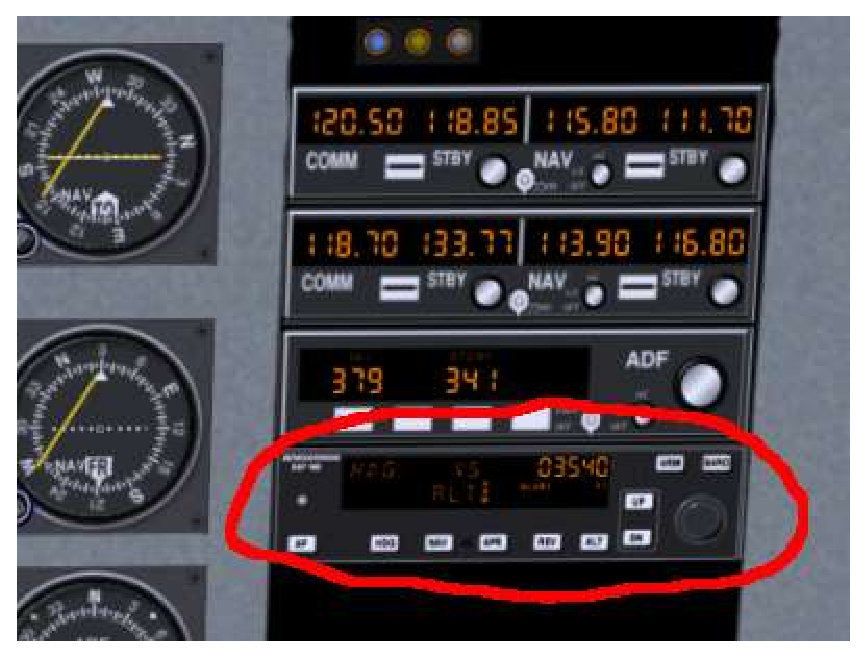
\includegraphics[width=0.5\textwidth]{autopilot}
\caption{C172 的自动驾驶仪\label{autopilot}}
\end{figure}

\Index{自动驾驶仪}面板在无线电栈的底层(如图~\ref{autopilot} 所示)。其上有很多按钮可以很容易的找到。自动驾驶仪可以工作在多种模式,我们这次只关注其中之一——HDG(航向模式)。正如其名字一样,HDG 模式会让飞机飞向之前我们在罗盘上设定航向游标所指示的航向。

要接通自动驾驶,只虚按 AP 按钮来打开自动驾驶,然后按 HDG 按钮激活航向模式。自动驾驶接通以后,会控制飞机调整片来调整飞机的航向。你可以修改航向游标,自动驾驶仪就会令飞机适实做出调整。然而自动驾驶仪并不会考虑风的影响,只会设定飞机的航向。如果是侧风飞行,飞机也许会指向某一点,但实际却偏差很大。

你需要使用调整片来保持水平飞行。也可以用自动驾驶仪来设置,不过会很复杂。

当飞机在自动驾驶仪的帮助下稳定下来以后,我们可以更多专注于外部世界,以及更高的技能。

\subsection{导航}

\begin{figure}[!htp]
\centering
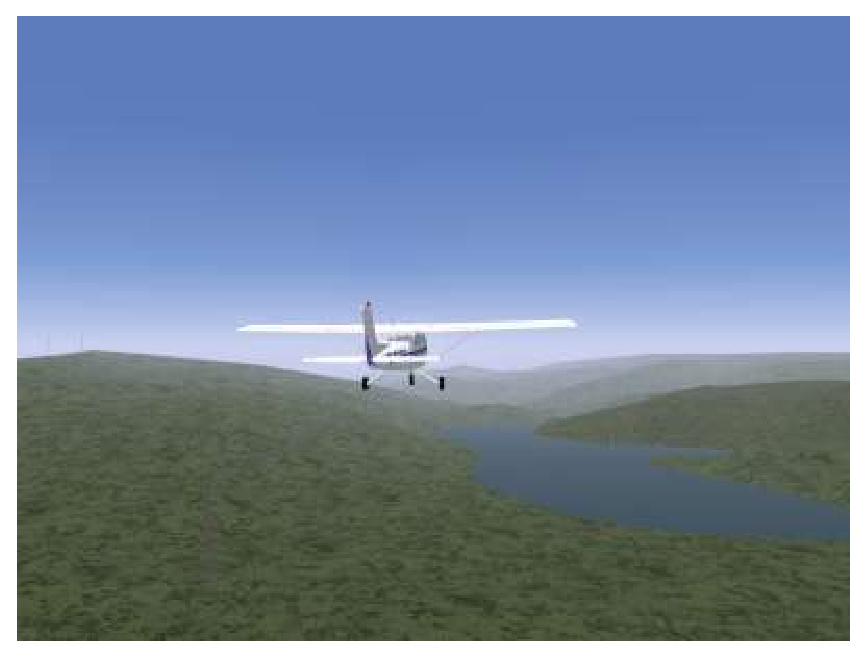
\includegraphics[width=0.5\textwidth]{calaveras1}
\caption{飞临卡拉韦拉斯水库}
\end{figure}

正如之前所说,我们会途径几个水库。起飞以后,首先涌入眼帘的也许是右手边的卡拉韦拉斯水库。你可以通过地图和地标来检查。如果感觉偏离航线,可以直接改变航向游标来修正。

\subsection{油气混合比}

\begin{figure}[!htp]
\centering
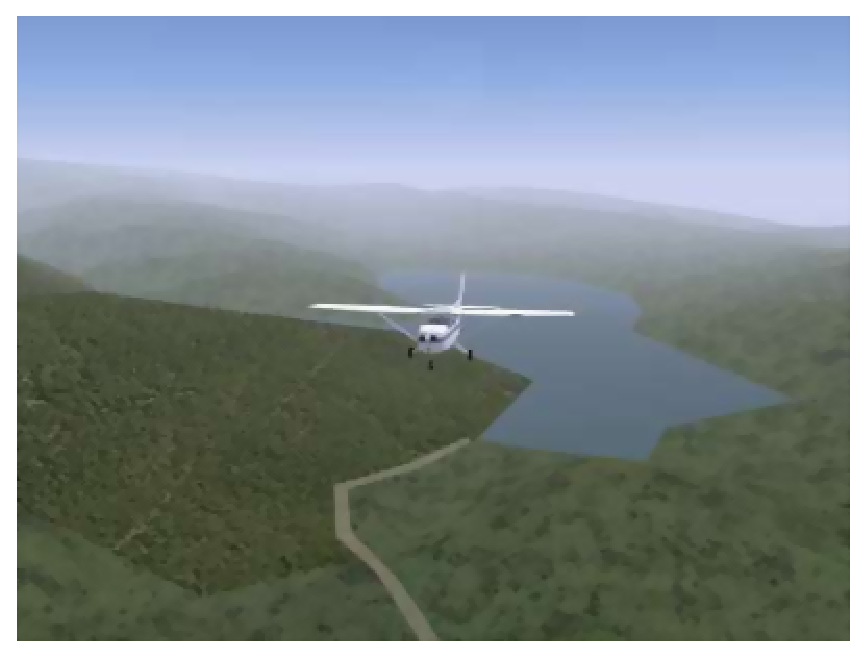
\includegraphics[width=0.5\textwidth]{calaveras2}
\caption{卡拉韦拉斯水库}
\end{figure}

随着高度的增加,空气越来越稀薄,氧气越来越少。这也就意味着发动机需要燃烧的燃油就减少了。C172 的发动机比较简单,没有配备自动燃油调整,以适应和修正氧气减少的情况。结果就会造成大量燃油消耗而动力却并不增加,因为油气混合比太多了(富油)。我可以通过\Index{油气混合比}控制杆控制燃油的配比。油气混合控制杆是油门杆旁边红色的那个,将杆向外拉表示“贫油”,即减小油气混合。我们不想让富油,也不想贫油,这种状态都不会有较高的动力输出。我们也不需要太完美,而只需要受控的燃烧即可,否则油气混合会产生爆炸,这很快就会把发动机报废。

\begin{figure}[!htp]
\centering
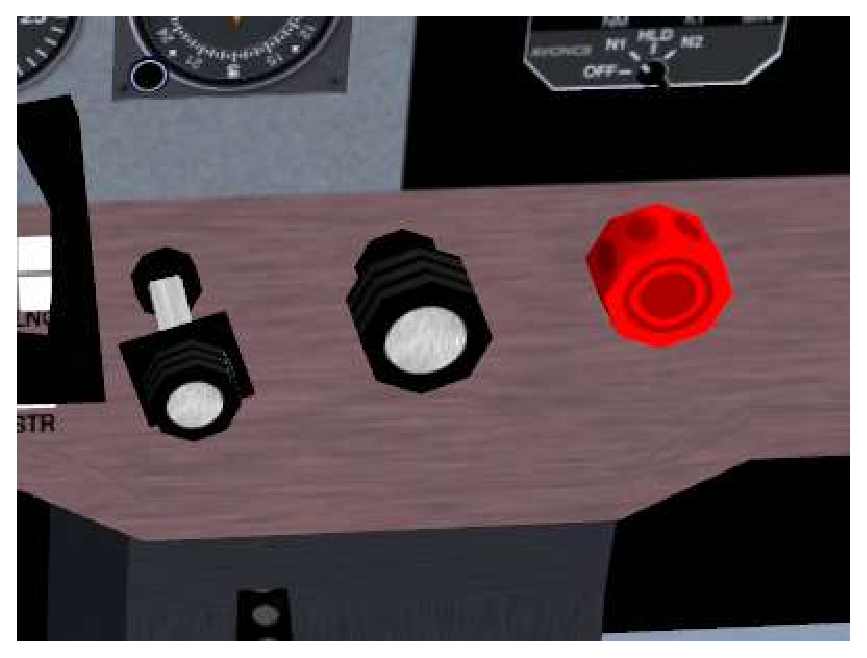
\includegraphics[width=0.5\textwidth]{mixture}
\caption{混合比控制\label{mixture}}
\end{figure}

用红色混合比杆来控制油气混合。你可能需要稍微移动一下视角才能看到它。

要移动视角,可以按住鼠标右键并移动鼠标。能看到油气混合比杆以后,就松开右键盘。

\begin{figure}[!htp]
\centering
\includegraphics[width=0.5\textwidth]{fuel_flow}
\caption{燃油流量和排气温度(EGT)指示计\label{egt}}
\end{figure}

轻轻向后拉油气混比(可以用 CTRL-C 观察可操作的热点),减少混合比。这样做可以观察到发动机的很多指标油了变化(主仪表板左侧)。燃油流量会下降(因为烧了更少的燃油),EGT(排气温度,Exhaust Gas Temperature)会上升(因为更接近“完美混合比”)并且 RPM 转速也会增加(会增加更多动力)。向外拉混合比杆,直到 EGT 表针超过量程,此时稍稍推混合比杆。现在我们在最佳富油状态。3500 英尺高度并不需要太贫的油,更高的高度适度贫油对发动机性能至关重要。

\section{下降阶段}

当我们抵达第二个水库(圣安东尼奥水库)的时候,我们要开始计划如何下降并降落在利弗摩尔。降落比起飞更复杂一些,如果你想一次性完成,此时可以先读完,并将模拟器暂停(按“p”键)。

\subsection{Air Traffic Control}

在真实飞行中,我们需要一直保持与\Index{空中交通管制}(ATC)的联通。正如湾区的地面交通一样,空中交通也很拥挤。ATC 会提供“飞行指引”服务,并会警告我们附近的飞机,防止在交汇时发生碰撞。FlightGear 的天空一般没有什么交通,因此我们也不需要飞行指引服务。如果你想修改空中交通的数量,可以从 AI 菜单找到。

利弗摩尔机场有塔台管制(塔台管制机场在区域图里以蓝色标出),因此我们需要联系塔台获取降落相关的信息。

在此之前,我们需要先收听机场通播(ATIS),并重新调整高度表拨正值,以防飞行过程中发生变化。短途飞行可能不会发生什么变化,但在数百英里的长途飞行中就有可能了。为了节省时间,可通过“设备”菜单的无线电设置对话框,输入相应的无线电频率。利弗摩尔机场的 ATIS 频率是 119.65 MHz。

ATIS 的信息以字母开头来标示信息序列,比如 Alpha(代表字母 A),Bravo(代表字母 B),…… Zulu(代表字母 Z)。此字母会在 ATIS 录音信息更新的时候变化。当联系塔台的时候,你需要告知你收到的 ATIS 信息标号,这样塔台可以双向检查飞行员是否获悉最新的机场信息。

除了高度表拨正值和天气状况,ATIS 也会告知正在使用的跑道,可以帮助我们计划降落。正常情况下,因为强劲的西风,利弗摩尔通常使用 25L 和 25R 跑道。

当你获悉 ATIS 以后,就可以将频率调到利弗摩尔机场的塔台了,频率是 118.1 MHz。取决于你设置的 AI 交通情况,你可能会听到塔台与其他正在起降的飞机之间的通话。这些信息并不会通过扬声器放出来,只会看到屏幕上的字幕。

当频道里安静以后,按“\` ”键打开 ATC 菜单。在左侧无线电按钮上选择你打算对塔台说什么(目前只有一个选项),然后点确认。

你的通话将会在屏幕上方显示出来。通话信息会包括你是谁(机型以及尾号),你在哪(比如,机场以南 6 海里),正打算落地,以及你收到的 ATIS 编号。

数秒之后,利弗摩尔机场塔台就会回应,会以名字称呼你并告诉你用哪条跑道,以及加入哪条起落航线,并告知何时联系他们。例如:

\begin{quote}
``Golf Foxtrot Sierra, Livermore Tower, Report left downwind runway two five left.''\footnote{这句话的意思是:GFS(表示飞机的呼号),利弗摩尔塔台,进入左转机场航线第三边时报告,使用 25L 跑道。——译者注}
\end{quote}

为了理解这句话,需要讲解一下机场起落航线\footnote{一般将 Traffic Pattern 翻译成“机场起落航线”(简称“起落航线“),或“五边航线”,此手册中出现类似情况都会按此翻译。——译者注}。

\subsection{起落航线}

机场周边会有很多飞机,必须有起飞和降落的标准流程,否则一架飞机可能会落在正在起飞的飞机头上。

\Index{起落航线}就是一个机场附近飞机必须遵守的标准航路,无论起飞还是降落。起落航线有四个阶段(或称四个“边”),如图~\ref{pattern} 所示。上文所说的“Downwind”(下风边,第三边),就表示的是图里标号为3的那一边。

\begin{figure}[!htp]
\centering
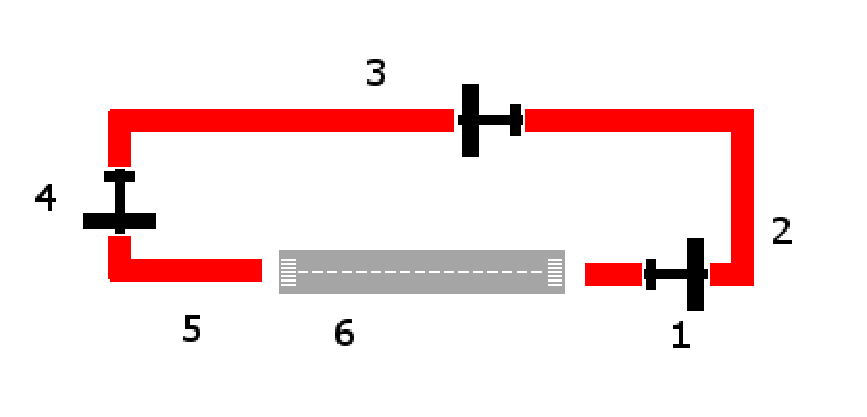
\includegraphics[width=0.5\textwidth]{pattern}
\caption{起落航线\label{pattern}}
\end{figure}

\begin{enumerate}
\item 飞机从跑道起飞和爬升时。如果正在离开机场,可以继续直线爬升直到脱离起落航线范围,之后做什么都行。如果要返回跑道(比如练习降落),就需要爬升到“起落航线高度”以下几百英尺的高度。此高度与地区差异有关,不过一般都是地面以上(AGL) 500 到 1000 英尺。也就是所谓的\emph{离场边(upwind,第一边)}。

\item 随后飞行员左转 90 度进入\emph{侧风边(Crosswind,第二边)}。他们会继续爬升到“起落航线高度”。

\item 在侧风边飞了 45 秒到一分钟以后,飞行员再向左转 90 度进入\emph{下风边(Downwind,第三边)}。此时很多从其他机场来此机场降落的飞机会加入,他们会以与跑道成 45 度角切入第三边。

\item 当飞过跑道尽头或一两英里(最好是跑道入口与你成 45 度角),随后飞行员再向左转 90 度进入\emph{基线边(Base,第四边)}并开始下降准备落地,适当放襟翼,下降率在 500 fpm 是比较合适的。

\item 45 秒之后飞行员转入\emph{最后进近(Final,第五边)}。这个转弯可能会较难以很精确对准跑道,最后降落时还需调整。我经常需要做小幅转弯以对准跑道。

\item 飞机落地,若飞行员正在练习起飞和降落,可以推油门并收襟翼来起飞,飞机就再次起飞了。这称为“Touch and Go”。

\end{enumerate}

大多数起落航线都是左手侧\footnote{因为飞行员坐在左侧,起落航线向左转有利于飞行员观察地形和其他飞机。——译者注},如上所说,所有转弯都是向左转。也有向右转的\footnote{若左侧起落航线会飞过人口稠密区,或其他不适宜飞机经过的地区,就会将起落航线设置为右手侧。——译者注}。在区域航图上会以“RP”标注。ATC 也会告诉你用何种起落航线。

\subsection{进近}

\begin{figure}[!htp]
\centering
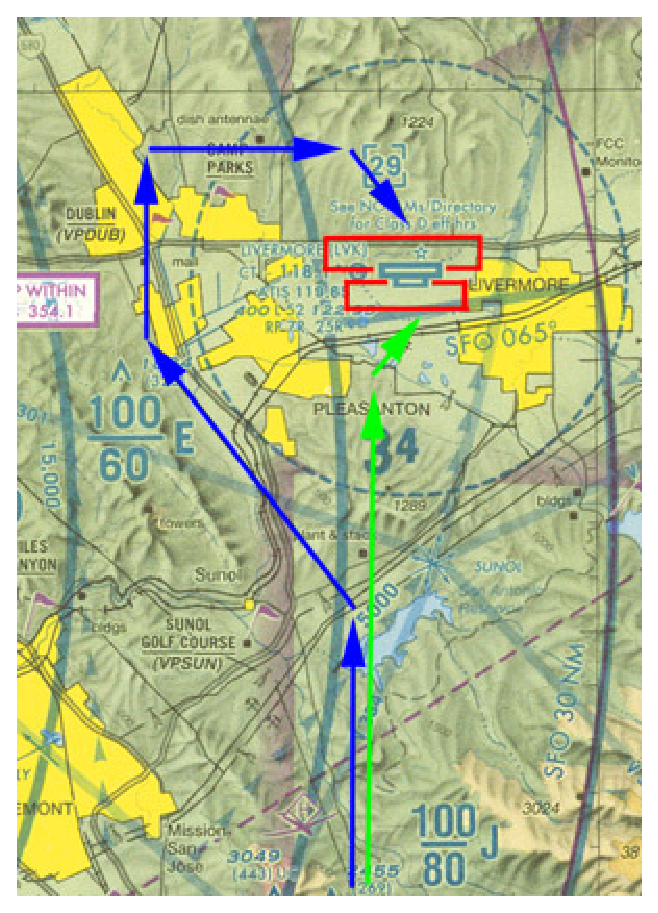
\includegraphics[width=0.5\textwidth]{livermore_pattern3}
\caption{从区域航图里摘抄出来的利弗摩尔进近航路\label{approach}}
\end{figure}

我们正在从南方接近利弗摩尔,因为盛行西风的关系,跑道是东西向的。我们需要使用 25L 或 25R 跑道落地,25R 用来做为右手侧起落航线的,而 25L 则是左手侧起落航线。两种起落航线都在图~\ref{approach} 里标出。取决于分配的跑道,我们需要用这两种起落航线之一。如果是用 25R 跑道落地,我们需要按上图中的蓝色线飞行;25L 跑道,则需要按绿色线飞行。

同时,我们需要降低高度,再加入起落航线时

%%%%%%%%%%%%%%%%%%%%%%%%%% ENGLISH VERSION %%%%%%%%%%%%%%%%%%%%%%%%%
\iffalse
\section{Introduction}

\begin{figure}[!htp]
\centering
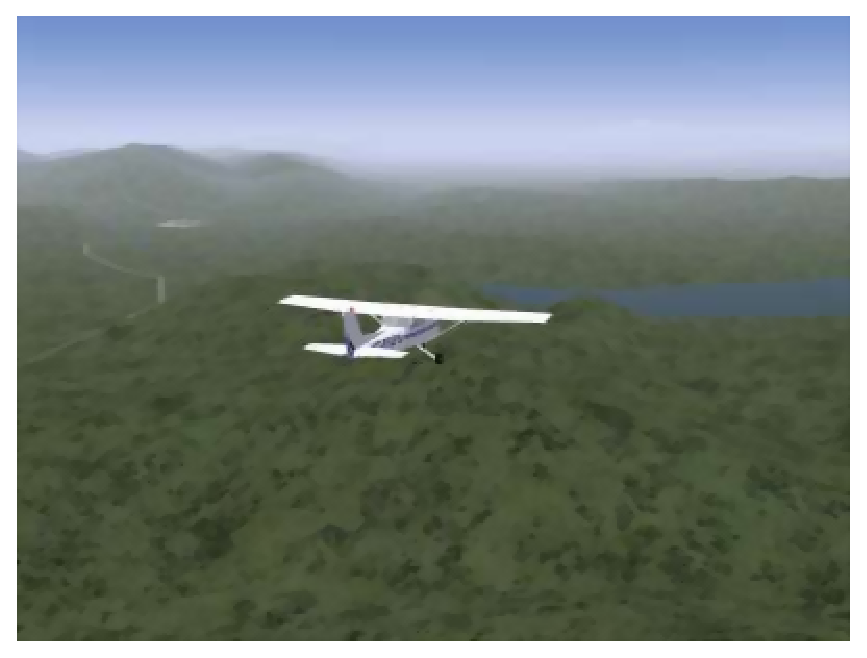
\includegraphics[width=0.5\textwidth]{antonio2}
\caption{Flying over the San Antonio Dam to Livermore}
\end{figure}

This tutorial simulates a cross-country flight from Reid-Hillview (KRHV) to
Livermore (KLVK) under Visual Flight Rules (VFR). Both airports are
included in the standard FlightGear package, so no additional scenery is required.

I'll assume that you are happy taking off, climbing, turning, descending
and landing in FlightGear. If not, have alook at the tutorials listed above.
This tutorial is designed to follow on from them and provide information on
some of the slightly more complicated flight systems and procedures.

\subsection{Disclaimer and Thanks}

A quick disclaimer. I fly microlights rather than Cessnas in real life. Most of
this information has been gleaned from various non-authoritive sources. If you
find an error or misunderstanding, please let me know. Mail me at
stuart\_d\_buchanan -at- yahoo.co.uk.

I'd like to thank the following people for helping make this tutorial accurate
and readable: Benno Schulenberg, Sid Boyce, Vassilii Khachaturov, James Briggs.

\section{Flight Planning}

Before we begin, we need to plan our flight.
Otherwise we'll be taking off not knowing whether to turn left or right.

First, have a look at the \Index{Sectional} for the area. This is a map for
flying showing airports, navigational aids, and obstructions.
There are two scales of sectionals for VFR flight -
the 1:500,000 sectionals themselves, and a number of
1:250,000 VFR Terminal Area Charts which cover particularly busy areas.

They are available from pilot shops, or on the web from various sources.
You can access a Google-map style interface here:

\medskip
\web{http://www.runwayfinder.com/}
\medskip

Simple search for Reid-Hillview. An extract from the chart is shown in Figure~\ref{sectional}.

\begin{figure}[!htp]
\centering
\includegraphics[width=\textwidth]{sectional}
\caption{Sectional extract showing Reid-Hillview and Livermore airports\label{sectional}}
\end{figure}

If you want a map of the entire area showing exactly where the plane is,
you can use Atlas.
This is a moving-map program that connects to FlightGear. See Section \ref{Atlas} for details.

So, how are we going to fly from Reid-Hillview to Livermore?

We'll be taking off from runway 31R at KRHV. KRHV is the ICAO code
for \Index{Reid-Hillview} airport, and is shown in the FlightGear wizard.
(It is marked on the sectional as RHV for historic reasons.
To get the ICAO code, simply prefix a `K'.)

The 31 indicates that the magnetic heading of the runway is around 310 degrees,
and the R indicates that it's the runway on the right. As can be seen from the
sectional, there are two parallel runways at KRHV. This is to handle the large
amount of traffic that uses the airport. Each of the runways can be used in
either direction. Runway 31 can be used from the other end as runway 13.
So, the runways available are 13R, 13L, 31R, 31L. Taking off and landing
is easier done into the wind, so when the wind is coming from the North West,
runways 31L and 31L will be in use. The name of the runway is written in large
letters at the beginning and is easily seen from the air.

Once we take off we'll head at 350 degrees magnetic towards \Index{Livermore} (KLVK).
We'll fly at about 3,500ft about sea-level. This puts us at least 500ft above any
terrain or obstructions like radio masts on the way.

We'll fly over the Calaveras Reservoir then the San Antonio Reservoir. These are
both large bodies of water and we can use them as navigation aids to ensure we
stay on the right track.

Once we get about 10 miles out of Livermore (above the San Antonia Reservoir),
we'll contact the Livermore Air Traffic Control (ATC) to find out
where we should land. We'll then join the circuit and land.

\section{Getting Up}

OK, we know where we're going and how we'll get there. Time to get started.

Start FlightGear using the Wizard (or command-line if you prefer).
 We want to use a C172P and take off from runway 31R at Reid-Hillview of
 Santa Clara County (KRHV). Dawn is a nice time to fly in California.

If you want, you can fly in the current weather at KRHV by clicking the
Advanced button on the final screen of the Wizard, selecting Weather
from the left-hand pane, selecting `Fetch real weather' and clicking OK.

\begin{figure}[!htp]
\centering
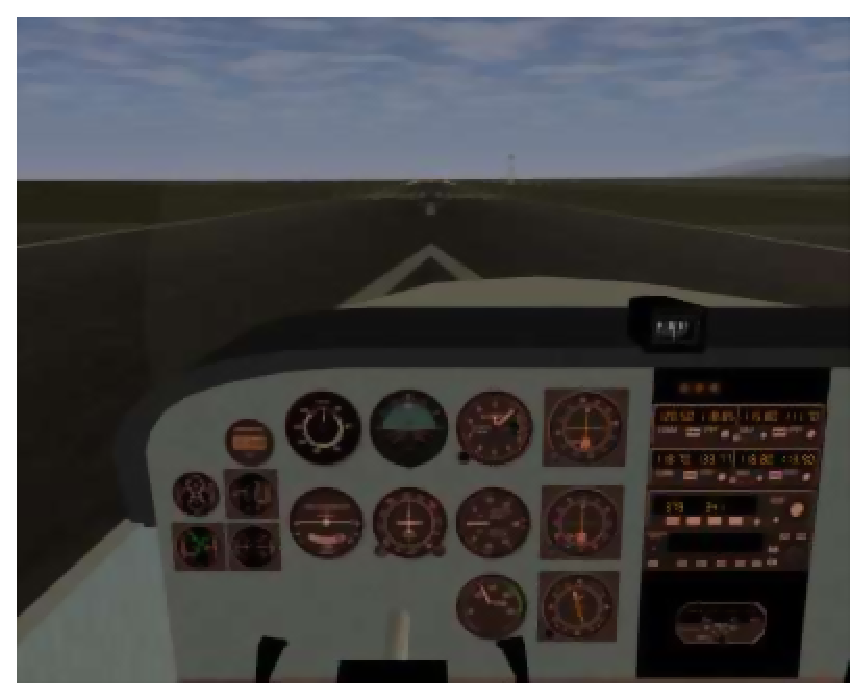
\includegraphics[width=0.5\textwidth]{krhvrunway}
\caption{On the runway at KRHV}
\end{figure}

\subsection{Pre-Flight}

Before we take off, we need to pre-flight the aircraft. In the real world,
this consists of walking around the aircraft to check nothing has fallen
off, and checking we have enough fuel.

In our case, we'll take the opportunity to check the weather, set our
altimeter and pre-set things that are easier to do when you're not flying.

The weather is obviously important when flying. We need to know if
there is any sort of cross-wind that might affect take-off, at what
altitude any clouds are (this is a VFR flight - so we need to stay
well away from clouds at all times), and any wind that might blow us off course.

We also need to calibrate our altimeter. Altimeters calculate the
current alititude indirectly by measuring air pressure, which decreases
as you ascend. However, weather systems can affect the air pressure and
lead to incorrect altimeter readings, which can be deadly if flying in mountains.

\subsection{ATIS}

Conveniently, airports broadcast the current sea-level pressure along
with useful weather and airport information over the \Index{ATIS}.
This is a recorded message that is broadcast over the radio.
However, to listen to it, we need to tune the radio to the correct frequency.

The ATIS frequency is displayed on the sectional (look for `ATIS' near the airport), but is also
available from within FlightGear. To find out the frequencies for an
airport (including the tower, ground and approach if appropriate),
use the ATC/AI menu and select Frequencies. Then enter the ICAO code
(KRHV) into the dialog box. The various frequencies associated with the
airport are then displayed. Duplicates indicate that the airport uses
multiple frequencies for that task, and you may use either.

Either way, the ATIS frequency for Reid-Hillview is 125.2MHz.

\subsection{Radios}

We now need to tune the \Index{radio}. The radio is located in the Radio
Stack to the right of the main instruments. There are actually two
independent radio systems, 1 and 2.  Each radio is split in two,
with a communications (COMM) radio on the left, and a navigation
(NAV) radio on the right. We want to tune COMM1 to the ATIS frequency.

\begin{figure}[!htp]
\centering
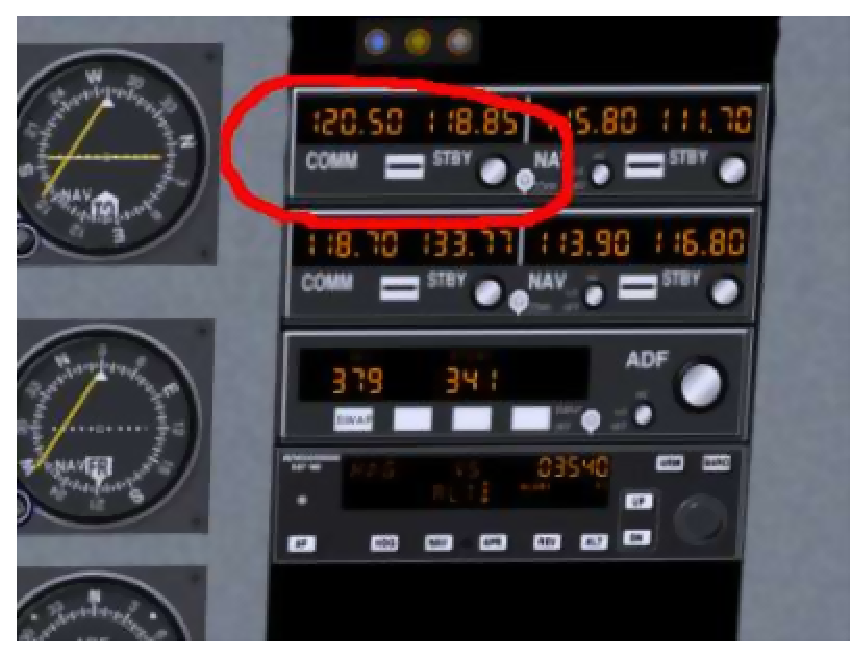
\includegraphics[width=0.5\textwidth]{comm1}
\caption{The C172 communications stack with COMM1 highlighted\label{comm1}}
\end{figure}

The radio has two frequencies, the active frequency, which is currently in use,
and the standby frequency, which we tune to the frequency we wish to use next.
The active frequency is shown on the left 5 digits, while the standby frequency
is shown on the right. We change the standby frequency, then swap the two over,
so the standby becomes active and the active standby. This way, we don't lose
radio contact while tuning the radio.

\begin{figure}[!htp]
\centering
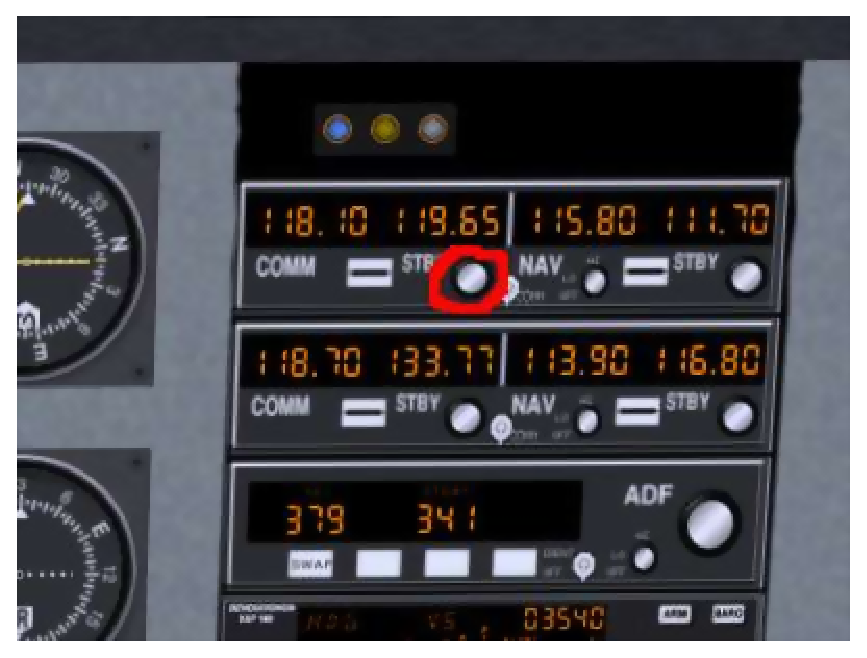
\includegraphics[width=0.5\textwidth]{comm1_knob}
\caption{COMM1 adjustment knob\label{comm1knob}}
\end{figure}

To change the frequency, click on the grey knob below the standby frequency
(highlighted in Figure~\ref{comm1knob}), just to the right of the `STBY'.
Using the left mouse button changes the number after the decimal place,
using the middle button changes the numbers before the decimal place.
Click on the right side of the button to change the frequency up, and
the left of the button to change the frequency down. Most of the FlightGear
cockpit controls work this way. If you are having difficulty clicking on the
correct place, press Ctrl-C to highlight the hot-spots for clicking.

\begin{figure}[!htp]
\centering
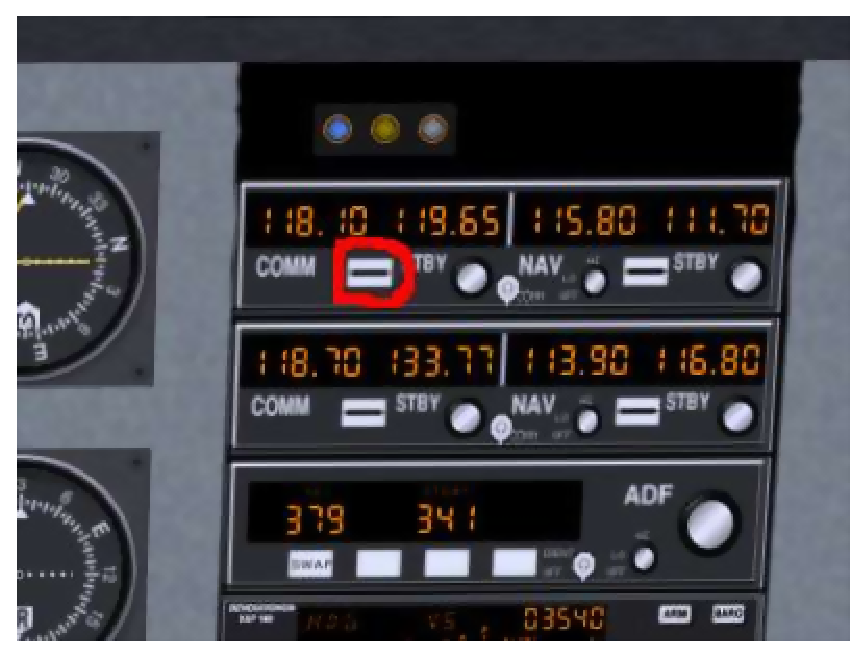
\includegraphics[width=0.5\textwidth]{comm1_switch}
\caption{COMM1 switch\label{comm1switch}}
\end{figure}

Once you have changed the frequency to 125.2, press the white button between
the words `COMM' and `STBY' to swap the active and standby frequencies
(highlighted in Figure~\ref{comm1switch}). After a second or so, you'll hear the ATIS information.

\subsection{Altimeter and Compass}

\begin{figure}[!htp]
\centering
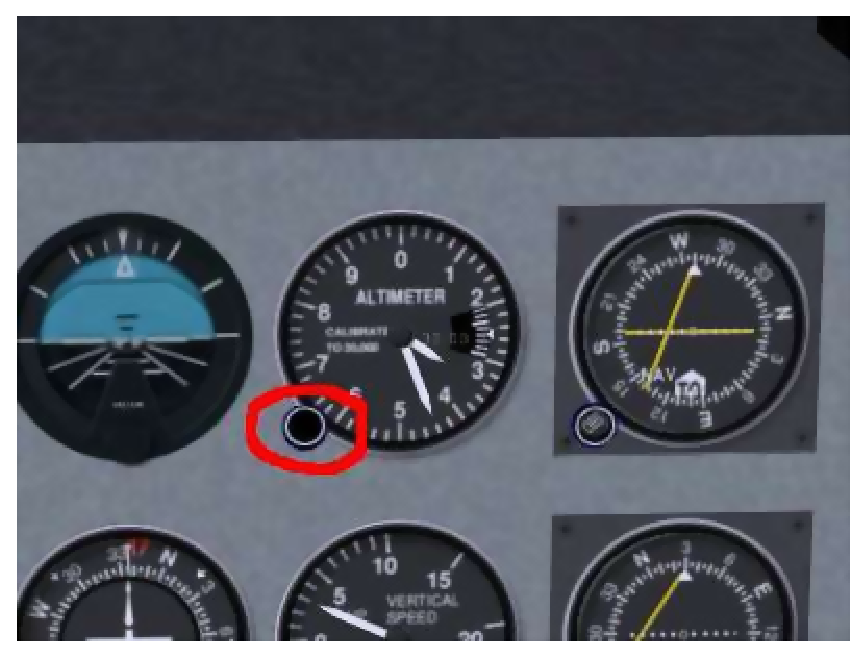
\includegraphics[width=0.5\textwidth]{altimeter}
\caption{Altimeter calibration knob\label{altimeter}}
\end{figure}

Listen for the `\Index{Altimeter}' setting. If you are not using `real weather',
the value will be 2992, which is standard and already set on the plane.
If you are using `real weather', then the altimeter value is likely to be different.
We therefore need to set the altimeter to the correct value.
To do this, use the knob at the bottom left of the altimeter
(circled in red in Figure~\ref{altimeter}), in the same way as
you changed the radio frequency. This changes the value in the
little window on the right of the altimeter, which is what you are
trying to set, as well as the altitude displayed by the altimeter.

The other way to set the altimeter is to match it to the elevation above
sea-level of the airport. The elevation is listed on the sectional.
For KRHV it is 133ft. This means you can double-check the pressure value reported over ATIS.

\begin{figure}[!htp]
\centering
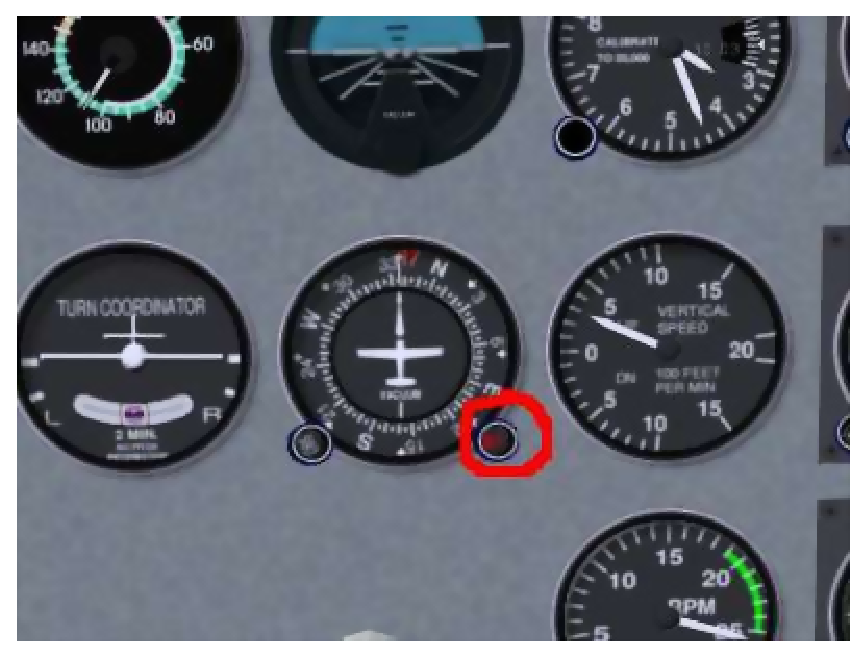
\includegraphics[width=0.5\textwidth]{compass}
\caption{Heading adjust knob\label{head}}
\end{figure}

We will also take the opportunity to set the heading bug on the compass to 350 -
our bearing from KRHV to KLVK. To do this, use the red button on the compass
housing (highlighted in Figure~\ref{head}), just as you've done before.
Use the left mouse button for small adjustments, and middle mouse button
to make big adjustments. The value of 350 is just anti-clockwise of the
labeled value of N (North - 0 degrees).

\begin{figure}[!htp]
\centering
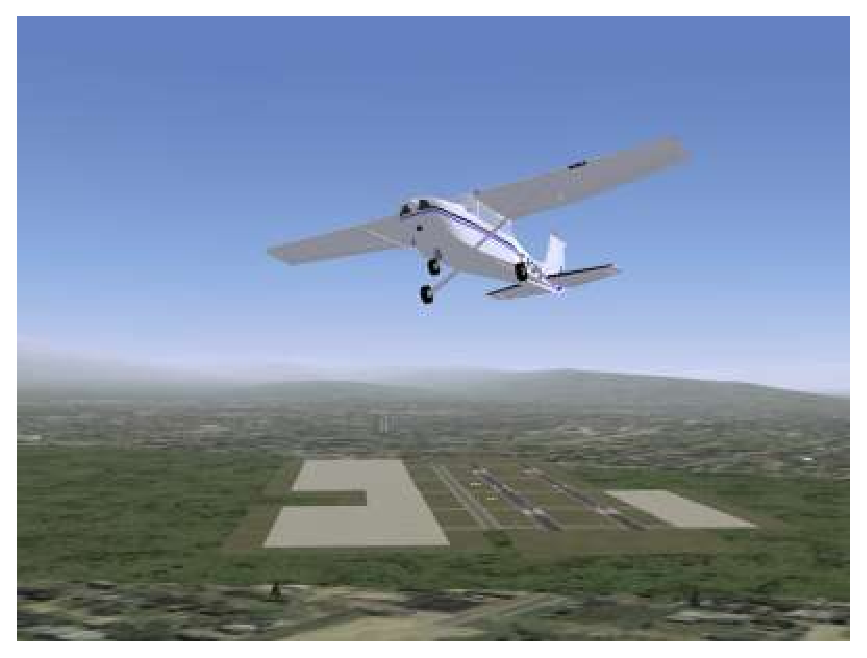
\includegraphics[width=0.5\textwidth]{takeoff}
\caption{Take-off from KRHV}
\end{figure}

\subsection{Take-Off}

OK, now we've done that we can actually take off!. In my case this usually
involves weaving all over the runway, and swerving to the left once
I've actually left the ground, but you'll probably have better control than me.
Once above 1000ft, make a gentle turn to the right to a heading of 350 degrees.
As we've set the heading bug, it will be easy to follow. We're aiming for a fairly prominent valley.


Continue climbing to 3,500 ft at around 500-700 fpm. Once you reach that altitude,
reduce power, level off to level flight and trim appropriately. Check the power
again and adjust so it's in the green arc of the RPM guage. We shouldn't run the
engine at maximum RPM except during take-off.

\section{Cruising}

OK, we've taken off and are on our way to Livermore. Now we can make our life a
bit easier by using the autopilot and our plane more fuel efficient by tuning
the engine. We'll also want to check we're on-course

\subsection{The Autopilot}

\begin{figure}[!htp]
\centering
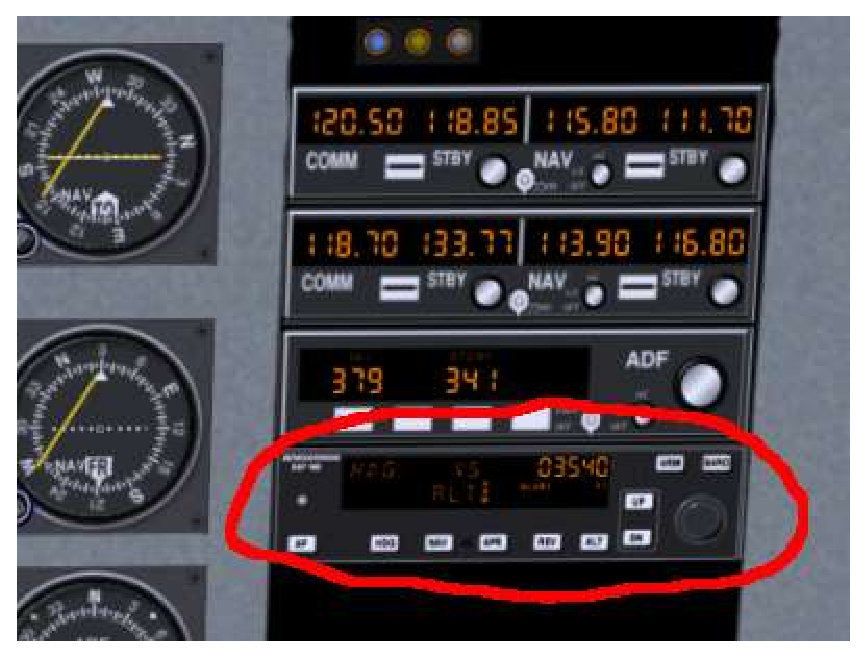
\includegraphics[width=0.5\textwidth]{autopilot}
\caption{The C172 Autopilot\label{autopilot}}
\end{figure}

We can make our life a bit easier by handing some control of the aircraft over
to `George' - the \Index{autopilot}.

The autopilot panel is located towards the bottom of the radio stack
(highlighted in Figure~\ref{autopilot}). It is easily distinguishable as
it has many more buttons than the other components on the stack. It can
work in a number of different modes, but we are only interested in one of
them for this flight - HDG. As the names suggest, HDG will cause the
autopilot to follow the heading bug on the compass, which we set earlier.

To set the autopilot, press the AP button to switch the autopilot on,
then press the HDG button to activate heading mode. While the autopilot
is switched on, it will use the trim controls to keep the
plane on the heading. You can change the heading bug, and the autopilot
will maneuver appropriately. However, the autopilot doesn't make any
allowances for wind speed or direction, it only sets the heading of
the airplane. If flying in a cross-wind, the plane may be pointed in
one direction, but be travelling in quite another.

You should use the trim controls to keep a level flight. You can use
the autopilot for this, but it is a bit more complicated.

Once the aircraft has settled down under the autopilot's control, we
can pay more attention to the outside world and higher level tasks.

\subsection{Navigation}

\begin{figure}[!htp]
\centering
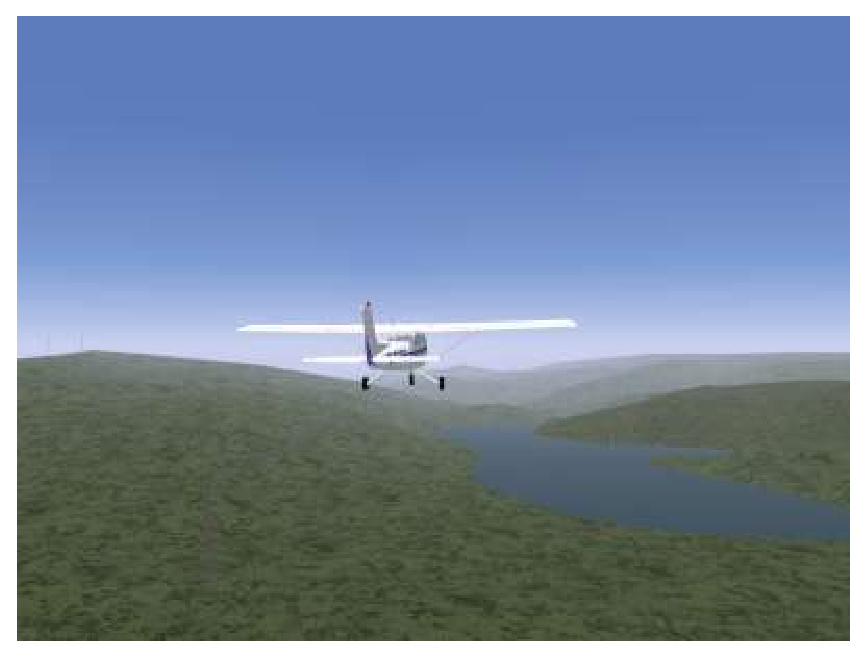
\includegraphics[width=0.5\textwidth]{calaveras1}
\caption{The Calaveras Reservoir}
\end{figure}

As we noted above, we're going to be travelling over a couple of reservoirs.
When you leveled off, the first (Calaveras) was probably right in front of you.
You can use them to check your position on the map. If it looks like you're
heading off course, twist the heading bug to compensate.

\subsection{Mixture}

\begin{figure}[!htp]
\centering
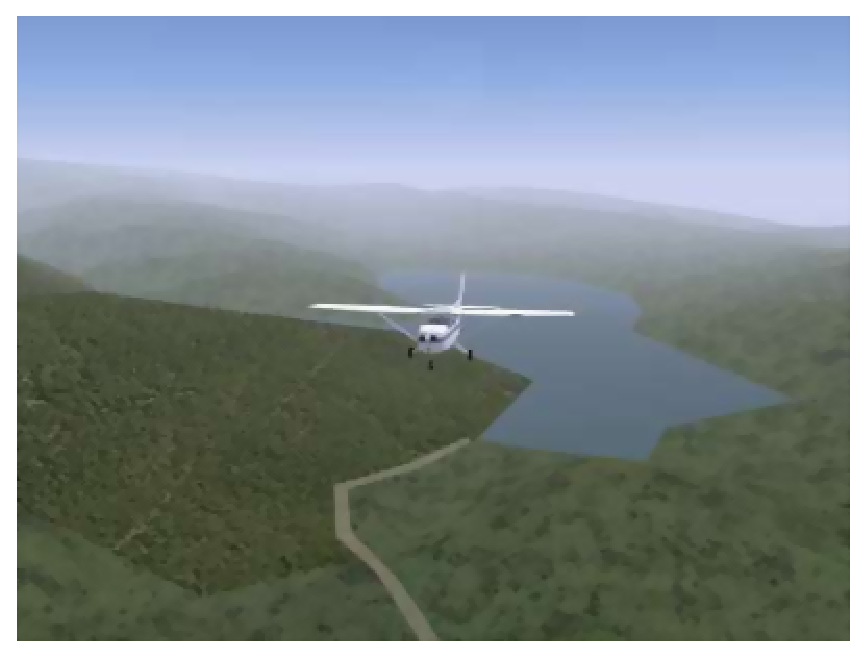
\includegraphics[width=0.5\textwidth]{calaveras2}
\caption{The Calaveras Reservoir}
\end{figure}

As altitude increases, the air gets thinner and contains less oxygen.
This means that less fuel can be burnt each engine cycle.
The engine in the C172 is simple and doesn't automatically
adjust the amount of fuel to compensate for this lack of oxygen.
This results in an inefficient fuel burn and a reduction in power
because the fuel-air mixture is too `rich'. We can control the
amount of fuel entering the engine every cycle using the \Index{mixture} control.
This is the red lever next to the throttle. By pulling it out, we `lean'
the mixture. We don't want the mixture too rich, nor too lean.
Both these conditions don't produce as much power as we'd like.
Nor do we want it perfect, because this causes the fuel-air to explode,
rather than burn in a controlled manner, which is a quick way to trash an engine.

\begin{figure}[!htp]
\centering
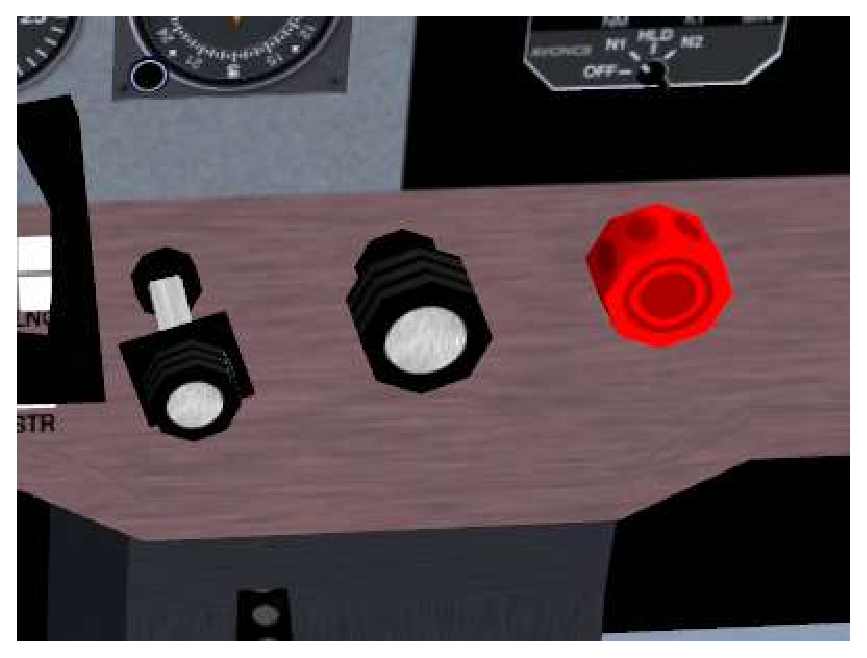
\includegraphics[width=0.5\textwidth]{mixture}
\caption{Mixture Control\label{mixture}}
\end{figure}

The mixture is controlled by the red lever to the right of the yoke.
You may need to pan your cockpit view to see it.

To pan the cockpit view, hold down the right mouse button Moving the mouse now
pans the view. Once you can see the mixture lever clearly, release the right
mouse button.

\begin{figure}[!htp]
\centering
\includegraphics[width=0.5\textwidth]{fuel_flow}
\caption{Fuel Flow and EGT guages\label{egt}}
\end{figure}

Pull the mixture lever out slowly (use Ctrl-C to see the hot spots),
leaning the mixture. As you do so, you'll see various engine instruments
(on the left of the panel) change. Fuel flow will go down (we're burning
less fuel), EGT (Exhaust Gas Temperature) will go up (we're getting closer
to a `perfect mixture') and RPM will increase (we're producing more power).
Pull the mixture lever out until you see the EGT go off the scale, then
push it in a bit. We're now running slightly rich of peak. While at
3,500ft we don't need to lean much, at higher altitudes leaning the
engine is critical for performance.

\section{Getting Down}

Once you reach the second reservoir (the San Antonio Reservoir),
we need to start planning our descent and landing at Livermore.
Landing is a lot more complicated than taking off, assuming you
want to get down in one piece, so you may want to pause the
simulator (press `p') while reading this.

\subsection{Air Traffic Control}

In the Real World, we'd have been in contact with \Index{Air Traffic Control} (ATC)
continually, as the bay area is quite congested in the air as well as on the ground.
ATC would probably provide us with a `flight following' service, and would continually
warn us about planes around us, helping to avoid any possible collisions.
The FlightGear skies are generally clear of traffic, so we don't need a flight following service.
If you want to change the amount of traffic in the sky, you can do so from the AI menu.

Livermore Airport is Towered (towered airports are drawn in blue on the sectional),
so we will need to communicate with the tower to receive instructions on how and where to land.

Before that, we should listen to the ATIS, and re-adjust our altimeter,
just in case anything has changed. This is quite unlikely on such a short flight,
but if flying hundreds of milesm it might make a difference. To save time when tuning
radios, you can access the Radio Settings dialog from the Equipment menu.
The Livermore ATIS frequency is 119.65MHz.

An ATIS message also has a phonetic letter (Alpha, Bravo, \ldots{} Zulu) to identify
the message. This phonetic is changed each time the recorded message is updated.
When first contacting a tower, the pilot mentions the identifier, so the tower can
double-check the pilot has up to date information.

Besides the altitude and weather information, the ATIS will also say which runway is in use.
This is useful for planning our landing. Normally, due to the prevalent Westerly wind,
Livermore has runways 25R and 25L in use.

Once you've got the ATIS, tune the radio to Livermore Tower. The frequency is 118.1MHz.
Depending on the level of AI traffic you have configured on your system, you may hear
Livermore Tower talking to other aircraft that are landing or departing.
This information is not played over the speakers, it is only displayed on the screen.

Once the frequency goes quiet, press the ' key. This will bring up the ATC menu.
Click on the radio button on the left to select what you wish to say (you only have one option), then OK.

Your transmission will be displayed at the top of the screen.
It will indicate who you are (type and tail number), where you are (e.g. 6 miles south),
that you are landing, and the ATIS you have.

After a couple of seconds, Livermore Tower will respond, addressing you by name and
telling you what runway to use, which pattern is in use and when to contact them, for example

\begin{quote}
``Golf Foxtrot Sierra, Livermore Tower, Report left downwind runway two five left.''
\end{quote}

To understand what this means, we'll have to describe the Traffic Pattern.

\subsection{The Traffic Pattern}

With the number of aircraft flying around, there have to be standard procedures
for take-off and landing, otherwise someone might try to land on-top of an aircraft taking off.

The \Index{Traffic Pattern} is a standard route all aircraft must follow when
near an airport, either taking off or landing. The traffic pattern has four
stages (or `legs'), shown in Figure~\ref{pattern}. The `downwind' mentioned
above refers to one of these, the one with the number 3.

\begin{figure}[!htp]
\centering
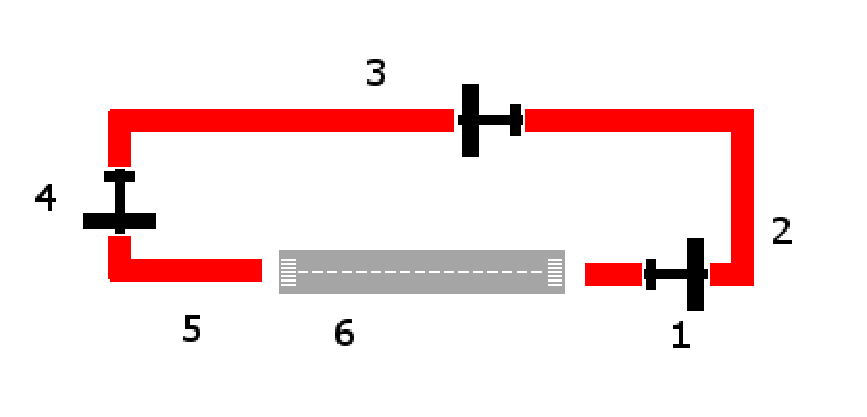
\includegraphics[width=0.5\textwidth]{pattern}
\caption{The Traffic Pattern\label{pattern}}
\end{figure}

\begin{enumerate}
\item Aircraft take off from the runway and climb. If they are leaving the
airport, they just continue climbing straight ahead until clear of the
pattern and then do whatever they like. If they are returning to the runway
(for example to practise landing), they continue climbing until they reach a
couple of hundred feet below `pattern altitude'. This varies from country to
country, but is usually between 500ft and 1000ft Above Ground Level (AGL).
This is called the \emph{upwind} leg.

\item The pilot makes a 90 degree left-hand turn onto the \emph{crosswind} leg.
They continue their climb to `pattern altitude' and level out.

\item After about 45 seconds to a minute on the crosswind leg,
the pilot again makes a 90 degree left turn onto the \emph{downwind} leg.
Aircraft arriving from other airports join the pattern at this point,
approaching from a 45 degree angle away from the runway.

\item When a mile or so past the end of the runway (a good guide is when the
runway is 45 degrees behind you), the pilot turns 90 degrees again onto the
\emph{base} leg and begins the descent to the runway, dropping flaps as appropriate.
A descent rate of about 500fpm is good.

\item After about 45 seconds the pilot turns again onto the \emph{final} leg.
It can be hard to estimate exactly when to perform this turn.
Final adjustments for landing are made.
I usually have to make small turns to align with the runway properly.

\item The aircraft lands. If the pilot is practising take-offs and landings,
full power can be applied and flaps retracted for takeoff, and the aircraft
can take off once more. This is known as `touch-and-go'.

\end{enumerate}

Most patterns at left-handed, i.e. all turns are to the left, as described
above. Right-hand patterns also exist, and are marked as `RP' on the sectional.
ATC will also advise you what pattern is in use.

\subsection{Approach}

\begin{figure}[!htp]
\centering
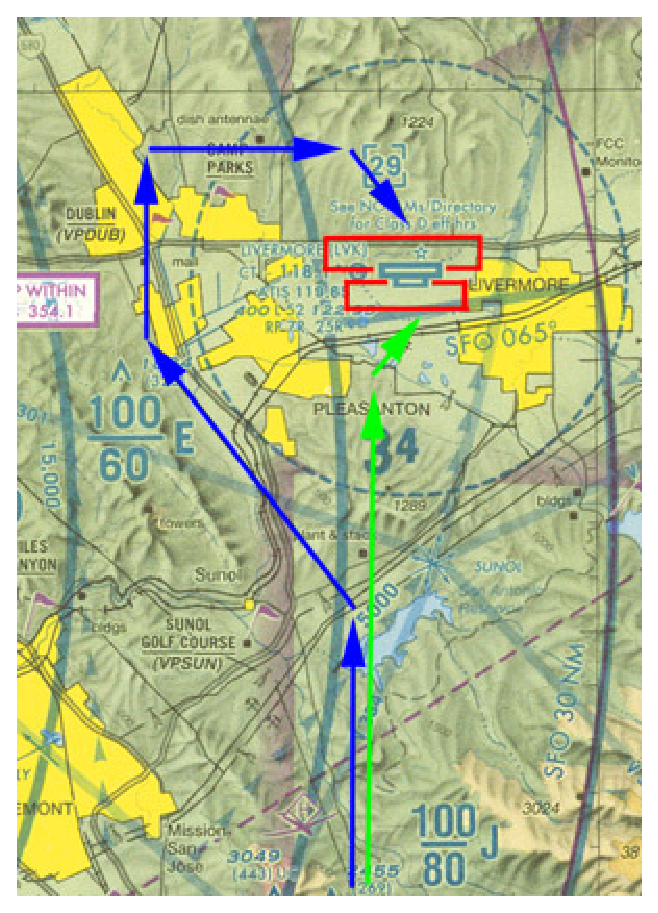
\includegraphics[width=0.5\textwidth]{livermore_pattern3}
\caption{Sectional extract showing approaches to Livermore\label{approach}}
\end{figure}

We're approaching Livermore airport from the South, while the runways run East/West.
Due to the prevailing Westerly wind, we'll usually be directed to either
runway 25R or 25L. 25R uses a right-hand pattern, while 25L uses a left-hand pattern.
Both the patterns are illustrated in Figure~\ref{approach}.
Depending on the runway we've been assigned, we'll approach the airport in one of two ways.
If we've been asked to land on runway 25R, we'll follow the blue line in the diagram.
If we've been asked to land on runway 25L, we'll follow the green line.

We also need to reduce our altitude. We want to end up joining the pattern at pattern
altitude, about 1,000ft above ground level (AGL). Livermore airport is at 400 ft above
sea-level (ASL), so we need to descend to an altitude of 1400 ASL.

We want to begin our maneuvers well before we reach the airport.
Otherwise we're likely to arrive too high, too fast, and probably
coming from the wrong direction. Not the best start for a perfect landing :).

So, let`s start descending immediately.

\begin{enumerate}
\item First switch off the autopilot by pressing the AP switch.

\item Return mixture to fully rich (pushed right in). If we were landing at a
high airport, we'd just enrich the mixture slightly and re-adjust when we reached the pattern.

\item Apply carb-heat. This stops ice forming when the fuel and air mix before
entering the cylinder, something that can often happen during descent in humid air.
The carb-heat lever is located between the throttle and mixture. Pull it out to apply heat.

\item Reduce power quite a bit. Otherwise we might stress the airframe due to over-speeding.

\item Drop the nose slightly to start the descent.

\item Trim the aircraft.

\end{enumerate}

Use your location relative to the airport and the two towns of Pleasanton and
Livermore to navigate yourself to the pattern following the general guide above.

Once you're established on the downwind leg, you'll need to report to ATC again.
Do this in the same way as before. They will then tell you where you are in the
queue to land. `Number 1' means there are no planes ahead of you, while
`Number 9' means you might want to go to a less busy airport! They'll also
tell you who is ahead of you and where. For example `Number 2 for landing,
follow the Cessna on short final' means that there is a single aircraft in
front of you that is currently on the final leg of the pattern. When they land and are
clear of the runway, they'll tell ATC, who can then tell you `Number 1 for landing'.

\subsection{VASI}

\begin{figure}[!htp]
\centering
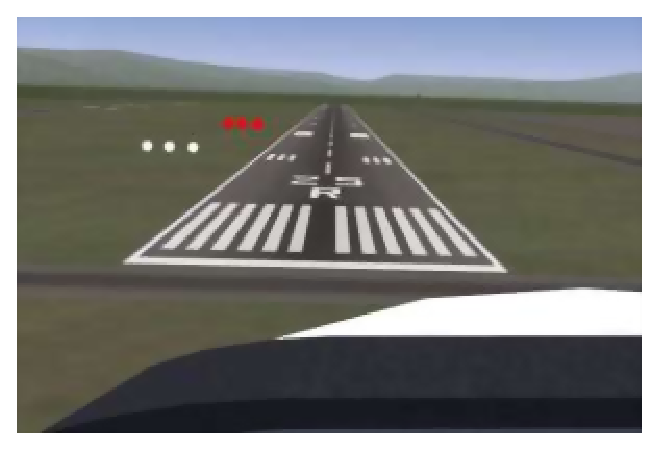
\includegraphics[width=0.5\textwidth]{vasi2}
\caption{On Final at Livermore with VASI on the left\label{vasi}}
\end{figure}

Once on final, you'll notice two sets of lights on the left of the runway
(enhanced in Figure~\ref{vasi}). This is the \Index{VASI} and provides a
nice visual clue as to whether you're too low or too high on approach.
Each set of lights can either be white or red. White means too high, red
means too low. White and red together means just perfect. On a Cessna
approaching at 60kts, a descent rate of about 500fpm should be fine.
If you are too high, just decrease power to increase your descent rate to
700fpm. If you are too low, increase power to decrease your descent rate to 200fpm.

\subsection{Go Around}

\begin{figure}[!htp]
\centering
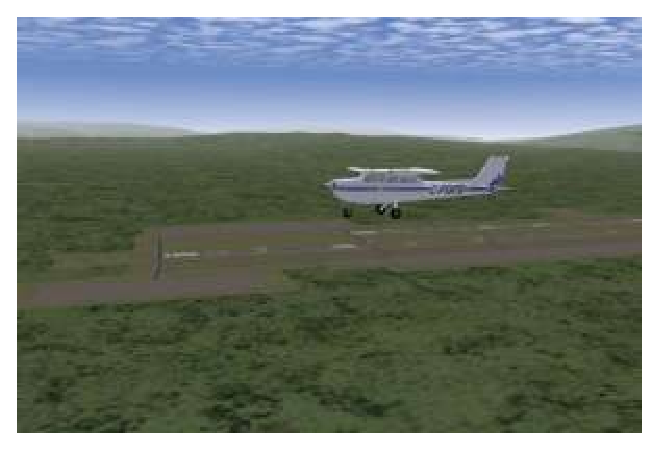
\includegraphics[width=0.5\textwidth]{missed}
\caption{Missed approach at Livermore}
\end{figure}

If for some reason it looks like you're going to mess up the landing
you can abort the landing and try again. This is called a `\Index{Go Around}'. To do this

\begin{enumerate}

\item Apply full power

\item Wait until you have a positive rate of climb - i.e.
your altitude is increasing according to the altimeter.

\item Raise your flaps to 10 degrees (first-stage).

\item Tell ATC you are `going around'

\item Climb to pattern height

\item If you aborted on final approach, continue over the runway to
re-join the pattern on the crosswind leg. If on base, fly past the
turn for final, then turn and fly parallel to the runway on the
opposite side from downwind to rejoin on the crosswind leg.

\item Fly the complete pattern, telling ATC when you are on downwind, and try again.

\end{enumerate}

\subsection{Clearing the Runway}

Once you're on the ground, you should taxi off the runway, then tell
ATC you are clear. At high-altitude airports, you would lean the engine to
avoid fouling the spark-plugs with an over-rich mixture.
Find somewhere nice to park, shut down the engine by pulling mixture to full lean,
then throttle off and magnetos to off (knob on the bottom left of the panel).
Switch off the avionics master switch, tie down the aircraft, then go get that hamburger!

I hope this tutorial is of some use. If you have any comments,
please let me know at stuart\_d\_buchanan \{at\} yahoo.co.uk.
\fi
